\chapter{Supplementary Material for Towards Universal Video Retrieval: Generalizing Video Embedding via Synthesized Multimodal Pyramid Curriculum}
\label{app:gve}

% \startcontents
% \printcontents{}{1}{\subsection*{Content}}

\section{Overview of Appendix}\label{gve:app:overview}
This appendix provides supplementary material supporting the main chapter, organized as follows:

\paragraph{Methodology Supplementary.}
\begin{itemize}
    \item \textbf{Details of Evaluations (for Section~\ref{gve:sec:uvrb}):} 
    (1)~\textit{UVRB Details (Appendix~\ref{gve:app:uvrb}):} Provides statistics, construction strategies, and evaluation details for all 16 datasets in UVRB.
    (2)~\textit{Evaluation Pipeline (Appendix~\ref{gve:app:evaluation_pipeline}):} Offers a technical overview of the scalable and reproducible evaluation protocol.
    
    \item \textbf{Details of Data Synthesis and Preparation (for Section~\ref{gve:sec:data_synthesis}):}
    (1)~\textit{Training Data (Appendix~\ref{gve:app:training_data}):} Details the composition and scale of the multi-modal training mixture.
    (2)~\textit{Dataset Construction Pipeline (Appendix~\ref{gve:app:data_construct}):} Explains the design principles of the unified dataset framework.
    (3)~\textit{Synthetic Data Prompts (Appendix~\ref{gve:app:prompt}):} Presents the structured prompts used for generating synthetic video retrieval data.
    
    \item \textbf{Details of Model and Training (for Section~\ref{gve:sec:modality_pyramid}):}
    (1)~\textit{Model Architecture (Appendix~\ref{gve:app:arch}):} Gives a detailed description of the GVE model architecture, including input fusion and embedding extraction.
    (2)~\textit{Training Implementation (Appendix~\ref{gve:app:hyperparameters}):} Outlines the parameter-efficient fine-tuning strategy and key hyperparameters.
\end{itemize}

\paragraph{Experimental Details and Results.}
\begin{itemize}
    \item \textbf{Baseline Details (Appendix~\ref{gve:app:baseline_details}):} Lists the specifications of all 14 evaluated baseline models.
    \item \textbf{Training Dynamics (Appendix~\ref{gve:app:training_dynamics}):} Visualizes training dynamics and metrics for the GVE-3B and GVE-7B models.
    \item \textbf{Additional Experiments}:
    \begin{itemize}
        \item[(1)] \textbf{Training-time Scaling (Appendix~\ref{gve:app:data_scaling}):} Presents the impact of scaling training data on performance, complementing the analysis in the main chapter.
        \item[(2)] \textbf{Test-time Scaling (Appendix~\ref{gve:app:scaling}):} Analyzes the effect of scaling test-time parameters (e.g., number of frames, resolution) on model performance.
        \item[(3)] \textbf{Data Quality Validation (Appendix~\ref{gve:app:v-synflow_validation}):} Details the human-in-the-loop evaluation conducted to validate the quality of our synthesized UVRD dataset.
        \item[(4)] \textbf{Curriculum Analysis (Appendix~\ref{gve:app:pyramid_validation}):} Provides in-depth experimental analysis to validate the design and effectiveness of the \pyramid.
        \item[(5)] \textbf{Video Classification (Appendix~\ref{gve:app:video_classification}):} Reports zero-shot classification performance on standard video action recognition benchmarks.
    \end{itemize}
\end{itemize}




\subsection{UVRB Details}\label{gve:app:uvrb}

This section provides details of UVRB  as shown in Figure~\ref{gve:fig:uvrb}, including statistics and construction strategies of datasets.

\begin{figure}[htbp]
    \centering
    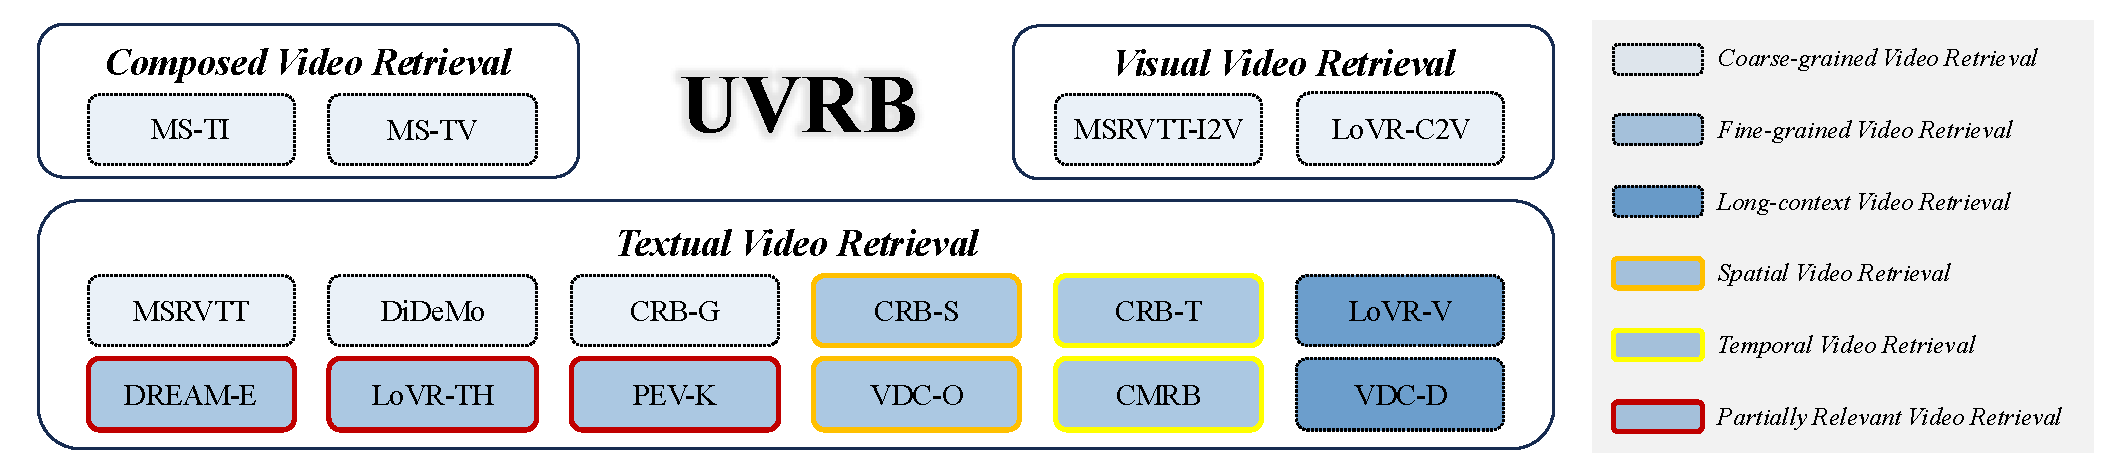
\includegraphics[width=\linewidth]{figures/gve/uvrb.pdf}
    \caption{The dataset category of Universal Video Retrieval Benchmark~(UVRB).}
    \label{gve:fig:uvrb}
\end{figure}

First, the statistics for the number of queries and corpus, the video durations, and the text lengths are presented in Table~\ref{gve:tab:uvrb_dataset}.

\begin{table}[htbp]
\centering
\caption{Statistics of datasets in the Universal Video Retrieval Benchmark (UVRB). All videos use 8 uniformly sampled frames. $\#$~Query: the number of queries; $\#$~Corpus: the number of corpus; Dur~(s):~Duration in seconds; $\#$~Word:~text length in words.}
\label{gve:tab:uvrb_dataset}
\begin{tabular}{l r r r r}
\toprule
\textbf{Dataset} & \textbf{$\#$~Query} & \textbf{$\#$~Corpus} & \textbf{Dur~(s)} & \textbf{$\#$~Word} \\
\midrule
\multicolumn{5}{l}{\textbf{Textual Video Retrieval~(Coarse-grained)}} \\
MSRVTT~\cite{xu2016msr} & 1,000 & 1,000 & 15.0 & 9.4 \\
DiDeMo~\cite{anne2017localizing} & 1,004 & 1,004 & 53.9 & 29.1 \\
CaReBench-General (CRB-G)~\cite{xu2025carebench} & 1,000 & 1,000 & 14.4 & 232.2 \\
\midrule
\multicolumn{5}{l}{\textbf{Textual Video Retrieval~(Fine-grained)}} \\
\multicolumn{5}{l}{\textbf{\textit{(a)~Spatial}}} \\
CaReBench-Spatial (CRB-S)~\cite{xu2025carebench} & 1,000 & 1,000 & 14.4 & 115.0 \\
VDC-Object~(VDC-O)~\cite{chai2024auroracap} & 1,027 & 1,027 & 30.1 & 91.4 \\
\multicolumn{5}{l}{\textbf{\textit{(b)~Temporal}}} \\
CaReBench-Temporal~(CRB-T)~\cite{xu2025carebench} & 1,000 & 1,000 & 14.4 & 103.2 \\
CameraBench~(CMRB)~\cite{lin2025towards} & 728 & 1,071 & 5.7 & 24.8 \\
\multicolumn{5}{l}{\textbf{\textit{(c)~Partially~Relevant}}} \\
DREAM-1K-Event~(DREAM-E)~\cite{wang2024tarsier} & 6,251 & 1,000 & 8.8 & 6.5 \\
LoVR-Theme2Clip~(LoVR-TH)~\cite{cai2025lovr} & 8,854 & 8,854 & 16.9 & 48.1 \\
PE-Video-Keyword~(PEV-K)~\cite{bolya2025perception} & 14,427 & 15,000 & 16.9 & 45.5 \\
\midrule
\multicolumn{5}{l}{\textbf{Textual Video Retrieval~(Long-context)}} \\
LoVR-Text2Video~(LoVR-V)~\cite{cai2025lovr} & 100 & 467 & 1560.3 & 17364.5 \\
VDC-Detail~(VDC-D)~\cite{chai2024auroracap} & 1,000 & 1,027 & 30.1 & 508.0 \\
\midrule
\multicolumn{5}{l}{\textbf{Composed Video Retrieval}} \\
MomentSeeker-Text-Image~(MS-TI)~\cite{yuan2025momentseeker} & 400 & 10 & 13.5 & 68.5 \\
MomentSeeker-Text-Video~(MS-TV)~\cite{yuan2025momentseeker} & 400 & 10 & 13.5 & 68.5 \\
\midrule
\multicolumn{5}{l}{\textbf{Visual Video Retrieval}} \\
MSRVTT-ImageVideo (MSRVTT-I2V)~\cite{xu2016msr} & 1,000 & 1,000 & 15.0 & - \\
LoVR-Clip-to-Video (LoVR-C2V)~\cite{cai2025lovr} & 467 & 467 & 1560.3 & - \\
\bottomrule
\end{tabular}
\end{table}

Second, we introduce the construction strategies of each dataset as follows.
\begin{itemize}
    \item~\textbf{MSRVTT:} We follow the data partition from JSFusion~\cite{yu2018joint}, utilizing 1,000 clip-text pairs from the original MSRVTT dataset~\cite{xu2016msr} for evaluation.

    \item~\textbf{DiDeMo:} Following the methodology in~\cite{liu2019use}, we concatenate all sentence descriptions associated with a single video from the DiDeMo dataset~\cite{anne2017localizing} to create a paragraph-level query for paragraph-to-video retrieval.

    \item~\textbf{CRB-G:} We adhere to the CaReBench protocol~\cite{xu2025carebench} and use the content from the \texttt{caption} field as the general query to retrieve videos.

    \item~\textbf{CRB-S:} Similar to CRB-G, we follow~\cite{xu2025carebench} and select the text from the \path{spatial_caption} field to form queries focused on spatial descriptions.

    \item~\textbf{VDC-O:} We utilize the VDC dataset~\cite{chai2024auroracap} and extract text from the \path{main_object_caption} field as an object-centric query (e.g., \textit{The main subject, a worker dressed in a gray sleeveless shirt and beige pants...}).

    \item~\textbf{CRB-T:} Similar to CRB-S, we again follow~\cite{xu2025carebench}, using the \path{temporal_caption} field to create queries based on temporal progression.

    \item~\textbf{CMRB:} We use the detailed camera motion annotations from CameraBench~\cite{lin2025towards} as queries to retrieve videos (e.g., \textit{The camera smoothly dollies forward, maintaining a steady and fluid motion...}).

    \item~\textbf{DREAM-E:} For event-based retrieval, we collect event descriptions from the DREAM-1K dataset~\cite{wang2024tarsier} to serve as queries for event-to-video matching (e.g., \textit{Wooden trap launches purple squirrel into the air}).

    \item~\textbf{LoVR-TH:} From the LoVR dataset~\cite{cai2025lovr}, we select the theme annotations of video clips as queries for theme-to-clip retrieval (e.g., \textit{The overall style of the animation is vibrant and whimsical...}).

    \item~\textbf{PEV-K:} We use the annotations from the \texttt{keyword} field in the PE-Video test set~\cite{bolya2025perception} to perform keyword-based partially relevant matching (e.g., \textit{colorful, paper, beautiful...}).

    \item~\textbf{LoVR-V:} We leverage the full-length video captions from the LoVR dataset~\cite{cai2025lovr} to perform long-text to long-video retrieval.

    \item~\textbf{VDC-D:} For this task, we extract the long, detailed descriptions from the \texttt{detailed\_caption} field of the VDC dataset~\cite{chai2024auroracap} to serve as fine-grained queries.

    \item~\textbf{MS-TI:} Following the adaptation method in~\cite{meng2025vlm2vec} for the MomentSeeker dataset~\cite{yuan2025momentseeker}, we create a text-image composed retrieval task. The goal is to retrieve a target video clip using a combined text and image query.

    \item~\textbf{MS-TV:} Similar to MS-TI, the task for MS-TV is to use a composed query of a text description and a reference video clip to retrieve the target clip.

    \item~\textbf{MSRVTT-I2V:} We construct image-to-video retrieval pairs from the aforementioned MSRVTT test set. For each video, a single frame is randomly sampled to serve as the image query for retrieving its source video.

    \item~\textbf{LoVR-C2V:} We leverage the original clip-to-video structure of the LoVR dataset~\cite{cai2025lovr}. For each full-length video, one of its corresponding short clips is used as the query for clip-to-video retrieval.
\end{itemize}

Third, we list the query prompt and metrics for datasets in evaluations in Table~\ref{gve:tab:uvrb_prompts_metric}.

\begin{table}[htbp]
\centering
\caption{Query Prompts and Metrics for Datasets in UVRB.}
\label{gve:tab:uvrb_prompts_metric}
\begin{tabular}{l p{9cm} l}
\toprule
\textbf{Dataset} & \textbf{Query Prompt} & \textbf{Metric} \\
\midrule
MSRVTT & Find the clip that corresponds to the described scene in the given video. & Recall@1 \\
DiDeMo & Find a video that includes the following described scenes. & Recall@1 \\
CRB-G & Find the video according to the general text description. & Recall@1 \\
CRB-S & Find the video according to the spatial description. & Recall@1 \\
VDC-O & Find the video according to the object description. & Recall@1 \\
CRB-T & Find the video according to the temporal description. & Recall@1 \\
CMRB & Find the video according to the camera motion description. & Recall@10 \\
DREAM-E & Find the video according to the text description. & Recall@1 \\
LoVR-TH & Find the video according to text description about video theme information. & Recall@10 \\
PEV-K & Find the video according to the text description of a series of keywords. & Recall@1 \\
LoVR-V & Find the long video according to the long text description. & Recall@1 \\
VDC-D & Find the video according to the detailed text description. & Recall@1 \\
MS-TI & Find the video clip that corresponds to the given text and the given image. & Precision@1 \\
MS-TV & Find the video clip that corresponds to the given text and the given video. & Precision@1 \\
MSRVTT-I2V & Find the video according to the image. & Recall@1 \\
LoVR-C2V & Find the original long video according to the short video clip. & Recall@1 \\
\bottomrule
\end{tabular}
\end{table}




\subsection{Evaluation Pipeline}\label{gve:app:evaluation_pipeline}
Our evaluation is built atop MTEB~\cite{muennighoff2022mteb}. It decouples the evaluation engine from model architecture—supporting everything from sentence transformers to custom multimodal encoders—via a standardized interface. The pipeline operates in three phases: (1) dynamic task orchestration, (2) configurable model execution, and (3) generation of metrics and diagnostics.
For instruction-sensitive tasks, it dynamically injects domain-specific prompts to mirror real-world conditions for actionable diagnostics.
Custom benchmarks are integrated seamlessly through dedicated loaders.
In this framework, expensive tasks are deferred for efficiency, model initialization (precision, multi-GPU) is abstracted via a factory, and data loading supports both online and offline modes for robustness across environments.
Engineering safeguards, including explicit multi-GPU management, clean shutdowns, and offline, first retry logic—ensure reliability at scale.




\subsection{Training Data}\label{gve:app:training_data}

To build a robust and versatile multimodal retrieval system, our models are trained on a large-scale, diverse mixture of text, image, and video data. All tasks are uniformly formulated as instruction-guided retrieval, a strategy designed to foster a unified representation space that can adeptly handle a wide array of queries. The training data is organized into two primary collections: a main mixture of widely-used public datasets (Table~\ref{gve:tab:main_training_data}), and a synthesized set from our Universal Video Retrieval Dataset (UVRD) suite (Table~\ref{gve:tab:uvrd_data}).

We follow existing works~\cite{li2023towards,Zhang_2025_CVPR} to construct text-only~(e.g., MSMARCO) and image-centric data~(e.g., CIRR).
In addition, we prepare video datasets using the following strategies.
\begin{itemize}
    \item \textbf{VAST}~\cite{chen2023vast}: We randomly select one sentence from the multiple vision captions as the text query for each video.
    \item \textbf{InternVid-FLT}~\cite{wang2023internvid}: We drop about $300$K low-quality videos and use the left text-video pairs.
    \item \textbf{PE-Video}~\cite{bolya2025perception}: We choose the $\text{human\_caption}$ refined on $\text{model\_caption}$ as the textual description of videos.
    \item \textbf{WebVid}~\cite{bain2021frozen}: We refuse the queries captioning over one video to impede the generality of text, which excludes $5$M videos in final training approximately.
\end{itemize}

\begin{table}[p]
\centering
\caption{Configuration of the main training data mixture for our 3B and 7B models. `K' denotes thousands, `M' denotes millions. Notes: (a) Task: T=Text, I=Image, V=Video. The format is Query→Corpus. (b) Neg.: Number of explicit hard negatives per positive. '0' indicates use of in-batch negatives only.}
\label{gve:tab:main_training_data}
\footnotesize
\begin{tabular}{@{}p{0.42\linewidth}crrcc@{}}
\toprule
\textbf{Dataset} & \textbf{Task} & \multicolumn{2}{c}{\textbf{Sample Size}} & \textbf{Neg.} & \textbf{BS} \\
\cmidrule(lr){3-4}
& & \textbf{3B} & \textbf{7B} & & \\
\midrule
\multicolumn{6}{l}{\textbf{Part 1: Text-only Data}} \\
MSMARCO & T→T & 300K & 500K & 2 & 64 \\
HotpotQA & T→T & \multicolumn{2}{c}{69K} & 1 & 64 \\
WebQA & T→T & \multicolumn{2}{c}{11K} & 1 & 32 \\
\midrule
\multicolumn{6}{l}{\textbf{Part 2: Image-centric Data}} \\
CIRR & TI→T & \multicolumn{2}{c}{16K} & 1 & 32 \\
Fashion200K & T→I & \multicolumn{2}{c}{4K} & 1 & 32 \\
Nights & I→I & \multicolumn{2}{c}{13K} & 1 & 32 \\
OVEN & TI→TI & 20K & 30K & 1 & 64 \\
OVEN & TI→T & 20K & 30K & 1 & 64 \\
VisualNews & T→I & 40K & 60K & 1 & 64 \\
EDIS & T→TI & \multicolumn{2}{c}{12K} & 1 & 32 \\
FashionIQ & TI→I & \multicolumn{2}{c}{4K} & 1 & 32 \\
MSCOCO & I→T & \multicolumn{2}{c}{4K} & 1 & 32 \\
REMUQ & TI→T & \multicolumn{2}{c}{5K} & 1 & 32 \\
WebQA & T→TI & \multicolumn{2}{c}{12K} & 1 & 32 \\
LLAVA & TI→T & 20K & 30K & 1 & 64 \\
EVQA & TI→TI & 20K & 30K & 1 & 64 \\
CC3M & T→I & 200K & 300K & 3 & 32 \\
CC3M & I→T & 100K & 200K & 2 & 64 \\
Laion & T→I & 300K & 500K & 3 & 32 \\
Laion & I→T & \multicolumn{2}{c}{200K} & 2 & 64 \\
ImageNet & I→T & 100K & 200K & 2 & 32 \\
VL3-Syn7M (short) & T→I & 300K & 500K & 3 & 32 \\
VL3-Syn7M (short) & I→T & 100K & 200K & 2 & 64 \\
VL3-Syn7M (detailed) & T→I & 200K & 300K & 3 & 32 \\
VL3-Syn7M (detailed) & I→T & 100K & 200K & 2 & 64 \\
VISTA & TI→I & \multicolumn{2}{c}{100K} & 2 & 32 \\
VISTA & T→TI & \multicolumn{2}{c}{20K} & 1 & 64 \\
\midrule
\multicolumn{6}{l}{\textbf{Part 3: Video-centric Data}} \\
VAST & T→V & \multicolumn{2}{c}{1.6M} & 0 & 32 \\
InternVid-FLT & T→V & \multicolumn{2}{c}{1.7M} & 0 & 32 \\
PE-Video & T→V & \multicolumn{2}{c}{104K} & 1 & 64 \\
WebVid & T→V & \multicolumn{2}{c}{5.4M} & 0 & 32 \\
\bottomrule
\end{tabular}
\end{table}

\begin{table}[htbp]
\centering
\caption{Configuration of UVRD. Sample sizes are identical for both 3B and 7B models. Notes: (a) Task: T=Text, I=Image, V=Video (Query→Corpus). (b) Neg.: Explicit hard negatives per positive. '0' denotes in-batch negatives only.}
\label{gve:tab:uvrd_data}
\begin{tabular}{l c c c c}
\toprule
\textbf{Dataset} & \textbf{Task} & \textbf{Size} & \textbf{Neg.} & \textbf{BS} \\
\midrule
UVRD-T2T & T→T & 100K & 0 & 64 \\
UVRD-T2I & T→I & 210K & 0 & 32 \\
UVRD-T2V & T→V & 879K & 1 & 64 \\
UVRD-TI2V & TI→V & 89K & 1 & 64 \\
UVRD-TV2V & TV→V & 35K & 1 & 64 \\
UVRD-I2V & I→V & 200K & 0 & 64 \\
UVRD-V2V & V→V & 36K & 0 & 64 \\
\bottomrule
\end{tabular}
\end{table}

As the aforementioned methodology, we train our model based on contrastive learning with pre-mined explicit hard negatives and in-batch negatives.
To maintain a balanced training diet and manage computational load, we employ a sophisticated data sampling strategy. For extremely large datasets, we sample a fixed number of instances. To amplify the learning signal from certain high-value or complex datasets, we may apply an upsampling strategy by repeating their data.

The scale of our training data is substantial. For our 3B parameter model, we prepared $12.55$ million instances. To further leverage the capacity of our 7B parameter model, we increase the sampling rate for several large-scale datasets, bringing the total instances to $13.73$ million. A detailed breakdown of the data composition is provided in Table~\ref{gve:tab:data_summary}.

\begin{table}[htbp]
\centering
\caption{Total number of instances for our 3B and 7B models across all data categories.}
\label{gve:tab:data_summary}
\begin{tabular}{@{}lrr@{}}
\toprule
\textbf{Data Category} & \multicolumn{2}{c}{\textbf{Total Sample Size}} \\
\cmidrule(lr){2-3}
& \textbf{3B Model} & \textbf{7B Model} \\
\midrule
Collected: Text-only & 380K & 580K \\
Collected: Image-centric & 1.82M & 2.80M \\
Collected: Video-centric & 8.80M & 8.80M \\
Synthesized: UVRD (All Modalities) & 1.55M & 1.55M \\
\midrule[1.5pt]
\bfseries Total & \bfseries 12.55M & \bfseries 13.73M \\
\bottomrule
\end{tabular}
\end{table}





\subsection{Dataset Construction Pipeline Details}\label{gve:app:data_construct}

Current multimodal retrieval research is hindered by fragmented, ad-hoc dataset construction. We introduce a unified, object-oriented framework that elevates this process to a rigorous science, balancing conceptual clarity with robustness for scalable, reproducible benchmarking.

The framework is anchored in a canonical tripartite abstraction: every retrieval task is decomposed into a \textsc{Corpus}, a set of \textsc{Queries}, and a \textsc{Relevance Mapping}. This schema, enforced by an abstract base class, is a conceptual invariant that ensures structural consistency across all datasets, from text-to-video to complex composed queries, enabling seamless model and evaluation compatibility.

The expressiveness of this data construction pipeline stems from polymorphic specialization via inheritance, encapsulated in three core strategies:

\paragraph{Modality as Configuration.}
Modality is a dynamic parameter. By overriding a single method, a dataset effortlessly transitions between modalities (text, image, video, or composite), transforming benchmarks like MSRVTT into image-to-video tasks with minimal code.

\paragraph{Task Derivation via Inheritance.}
Complex tasks are composed of simpler ones. A text+image-to-video task inherits its base structure and extends the query schema. Variants are derived by overriding specific data-access methods, turning benchmark creation into a modular, hypothesis-driven workflow.

\paragraph{Engineering for Scale and Integrity.}
Scalability and data quality are first-class principles. Large datasets (e.g., InternVid-FLT) leverage chunked, parallel processing. Crucially, proactive curation is embedded: automated validators check video integrity (resolution, frame count), while repair mechanisms fix common errors using \texttt{ffmpeg}, ensuring failures reflect retrieval challenges, i.e., not data corruption.









\subsection{Prompt for Synthetic Video Retrieval Data Generation}\label{gve:app:prompt}

To ensure high-quality, diverse, and controllable synthetic video retrieval data generation at scale, we design and deploy a suite of structured prompts to instruct MLLMs for captioning. Our pipeline operates in four parts:

\begin{enumerate}
    \item \textbf{Raw~(Or Weakly Annotated) Video (Re-)~Captioning}: Enhance raw or uncaptioned videos with rich, diverse textual descriptions.
    \item \textbf{Text-Image Composed Retrieval}: Generate queries that combine reference images with video content for fine-grained retrieval.
    \item \textbf{Text-Video Composed Retrieval}: Generate queries that combine short reference clips with target videos for practical temporal or perspective-based retrieval.
    \item \textbf{Frame Image Captioning}: Annotate individual video frames with dynamic-aware captions for auxiliary training signals.
\end{enumerate}

All prompts enforce strict output formatting, factual grounding, and stylistic diversity to ensure dataset quality and coverage. \texttt{\{raw\_caption\}} represents an optional, potentially low-quality human-provided or auto-generated caption associated with the video. Placeholders (e.g., \texttt{\{readability\}} and \texttt{\{education\_level\}}) are dynamically instantiated during batch generation.

Besides, we can generate text-to-text retrieval data from the multiple video/frame captions by randomly matching any two sentences in the caption list.

% ========================================
% Prompt 1: Video Captioning
% ========================================
\begin{promptbox}{Synthetic Video Captioning Prompt}
\begin{lstlisting}[style=promptstyle]
Generate 5 distinct and high-quality ENGLISH captions for the provided video. Please first visually understand the video file and analyze the video frame-by-frame in depth before captioning.

The original video caption is {raw_caption}. (Ignore if empty.)

Each caption must be:
  1. The final answer MUST only be a JSON dict of captions where the key is the caption number and the value is a single-paragraph caption.
  2. Factually accurate and descriptive - include only what is clearly visible or reasonably inferable from the video.
  3. Focus exclusively on visible content; do not mention absences or speculate about unseen elements.

Content Requirements (per caption):
  1. Spatial Details (30-60%): Describe location, setting, key environmental elements, objects, and their spatial relationships. Include notable visual features.
  2. Temporal Flow (30-60%): Capture event sequence and action dynamics - movements, interactions, transitions - as they unfold over time.
  3. Theme/Background/Style/Meaning/Highlight/Camera (0-20%): Describe observable emotional tone, narrative style, thematic elements, highlighting frames, or significant camera movements/angles.
  4. Others (0-10%).

Key Guidelines:
  1. Do not invent fictional elements, dialogue, or backstory not visible in the video.
  2. Use the following varied sentence styles (one per caption):
       - concise and punchy summary,
       - spatial-temporal richly descriptive,
       - abstract understanding,
       - keywords-only,
       - partially relevant information.
  3. Ensure diversity: avoid repetition in wording, focus, or rhythm; at least one caption must be <20 words and one >100 words; balance objectivity with vivid sensory language; randomly omit minor details in 1 or 2 captions.
  4. Ensure readability matches {readability} and is appropriate for {education_level} readers.

Now generate these captions in strict JSON format:
{
   "1": <caption text 1: concise and punchy summary, 10-25 words>,
   "2": <caption text 2: spatial-temporal richly descriptive, 80-200 words>,
   "3": <caption text 3: abstract understanding, 30-100 words>,
   "4": <caption text 4: keywords-only, 5-30 words>,
   "5": <caption text 5: partially relevant information, 10-70 words>
}
\end{lstlisting}
\end{promptbox}

% ========================================
% Prompt 2: Text-Image Composed Retrieval
% ========================================
\begin{promptbox}{Synthetic Text-Image Composed Video Retrieval Prompt}
\begin{lstlisting}[style=promptstyle]
You are an information retrieval expert specializing in high-value text-image composed queries. Your sole objective is to generate queries that significantly enhance video retrieval performance by effectively combining a reference image and video content.

## What Makes a HIGH-QUALITY Query (Non-Negotiable)
A truly valuable query must satisfy ALL of these criteria:

1. COMBINATION NECESSITY (Most Critical)
   - The query MUST become meaningless or significantly less specific if either the image or video is removed.
   - Example (HIGH-QUALITY): "the person FROM REFERENCE IMAGE wearing red jacket now skiing"
   - Example (LOW-QUALITY): "a person skiing" (works without image)

2. SEMANTIC PRECISION
   - Must accurately reflect BOTH the visual content of the reference image AND the video.
   - Must reference at least ONE specific visual attribute from the image (not generic descriptions).
   - Example (HIGH-QUALITY): "matching the blue hat FROM PHOTO, now running through park"
   - Example (LOW-QUALITY): "someone similar to image moving" (too vague)

3. RETRIEVAL EFFECTIVENESS
   - Must narrow search results by at least 50\% compared to text-only queries.
   - Must contain actionable constraints that differentiate from 90\% of videos in the database.
   - Example (HIGH-QUALITY): "the woman WITH PONYTAIL FROM IMAGE entering building at 2PM"
   - Example (LOW-QUALITY): "a woman walking" (too broad)

4. LOGICAL COHERENCE
   - Must maintain subject-verb-object consistency across modalities.
   - Must avoid semantic contradictions between image attributes and video actions.
   - Example (HIGH-QUALITY): "the dog FROM REFERENCE PHOTO chasing a ball"
   - Example (LOW-QUALITY): "the red jacket FROM IMAGE running down hill" (jackets don't run)

5. PRACTICAL UTILITY
   - Must solve a real-world ambiguity that neither text nor image could resolve alone.
   - Must reflect how actual users would express their information need.
   - Example (HIGH-QUALITY): "same person AS IN PHOTO but wearing blue instead of red"
   - Example (LOW-QUALITY): "the image shows a person and the video shows action" (no real combination)

## High-Value Query Generation Framework
Follow this structured approach:

1. DEEP ANALYSIS PHASE (Mandatory)
   a) Reference Image Analysis:
      - Identify 1-4 SPECIFIC visual attributes (e.g., "red jacket", "ponytail", "blue hat")
      - Determine primary subject with discriminative features
      - Note what CANNOT be determined from image (e.g., action, scene)
   
   b) Video Content Analysis:
      - Identify primary action using precise verbs (e.g., "running", "entering", "chasing")
      - Note scene context and temporal elements
      - Determine what CHANGES from the static image reference

2. COMBINATION STRATEGY SELECTION
   Choose ONE primary strategy:

   A) IDENTITY PRESERVATION + ACTION CHANGE
      - Structure: [Binding phrase] + [Image attribute] + [Video action]
      - Example: "the man FROM REFERENCE IMAGE in blue shirt now running"
   
   B) IDENTITY PRESERVATION + SCENE MIGRATION
      - Structure: [Binding phrase] + [Image attribute] + [Scene transition]
      - Example: "same person AS IN PHOTO moving from office to park"
   
   C) IDENTITY PRESERVATION + NEGATIVE CONSTRAINT
      - Structure: [Binding phrase] + [Negative constraint] + [Video state]
      - Example: "not wearing red jacket FROM IMAGE but blue, walking"
   
   D) RELATIONAL TRANSFER
      - Structure: [Binding phrase] + [Relationship description]
      - Example: "the dog FROM REFERENCE PHOTO chasing a ball"

3. QUALITY ENHANCEMENT TECHNIQUES
   - Binding Precision: Use "FROM REFERENCE IMAGE", not "like the picture"
   - Attribute Specificity: Use concrete features ("red jacket", not "clothing")
   - Action Verbs: Use present continuous tense ("running", not "runs")
   - Context Enrichment: Add 1 relevant scene descriptor ("in park", "near building")
   - Noise Handling: For low-quality inputs, use "resembling" but maintain specificity
   - Audience Adaptation: Ensure readability matches {readability} and suits {education_level} readers.

4. MANDATORY QUALITY CHECK
   Before finalizing, verify ALL:
   - [ ] Explicit binding to reference image
   - [ ] References SPECIFIC visual attribute from image
   - [ ] Describes DYNAMIC ELEMENT not in static image
   - [ ] Loses specificity if image removed
   - [ ] Contains actionable retrieval constraint
   - [ ] Maintains logical subject-action consistency
   - [ ] Solves real-world ambiguity

## What to AVOID
- Generic descriptions ignoring image specificity
- Redundant mentions of obvious image content
- Semantic contradictions (e.g., "the jacket is running")
- Overly precise details not visible in inputs
- Standalone video descriptions without image binding
- Vague terms: "something", "thing", "area"
- Excessive length without added value (>50 words)

## Output Format
- Output ONLY a JSON object with one key: "query"
- Value must be the generated query sentence
- No additional text or formatting

Generate the query for:
Reference Image: <image_input>
Video Clip: <video_input>
\end{lstlisting}
\end{promptbox}

% ========================================
% Prompt 3: Text-Video Composed Retrieval
% ========================================
\begin{promptbox}{Synthetic Text-Video Composed Video Retrieval Prompt}
\begin{lstlisting}[style=promptstyle]
You are an information retrieval expert specializing in practical text-video composed queries. Your objective is to generate queries that effectively combine a short reference clip with a target video for real-world retrieval.

## Practical Context Understanding
In real-world scenarios:
- Reference is typically a SHORT CLIP (2-10 seconds)
- Clip is usually HIGHLY RELEVANT to target video (same source or similar content)
- Common relationships: temporal continuation, perspective variation, quality differences, minor action variations
- Query should reflect how users actually search

## What Makes a HIGH-QUALITY Query (Practical Focus)
Must satisfy these criteria:

1. USEFUL COMBINATION (Most Important)
   - Leverages reference clip to specify what text alone cannot
   - Example (HIGH-QUALITY): "the same person FROM REFERENCE CLIP continuing to run after the jump"
   - Example (LOW-QUALITY): "a person running" (ignores reference)

2. PRACTICAL PRECISION
   - References at least ONE observable feature from reference clip
   - Example (HIGH-QUALITY): "matching the red jacket FROM REFERENCE, now entering building"
   - Example (LOW-QUALITY): "someone similar to clip moving" (too vague)

3. REAL-WORLD UTILITY
   - Helps find videos difficult to retrieve with text alone
   - Example (HIGH-QUALITY): "same action AS IN REFERENCE but from front angle"
   - Example (LOW-QUALITY): "the clip shows action" (no retrieval value)

4. NATURAL EXPRESSION
   - Sounds like how a real user would phrase it
   - Example (HIGH-QUALITY): "what happens right after this moment?"
   - Example (LOW-QUALITY): "temporal continuation of the current visual sequence" (too academic)

## Practical Query Generation Framework

1. REFERENCE CLIP ANALYSIS
   - Identify 1-3 KEY OBSERVABLE FEATURES (e.g., "red jacket", "starting pose", "mid-action")
   - Determine most distinctive visual or action element
   - Note what is CLEARLY VISIBLE (avoid guessing)

2. TARGET VIDEO RELATIONSHIP ASSESSMENT
   Determine relationship type:
   
   A) TEMPORAL CONTINUATION
      - Reference is earlier part of same sequence
      - Query focus: "what happens next" or "continuing action"
   
   B) PERSPECTIVE VARIATION
      - Same action from different angle/view
      - Query focus: "same action from different angle"
   
   C) QUALITY/CONDITION VARIATION
      - Same action with different lighting/resolution
      - Query focus: "same scene in better lighting"
   
   D) MINOR ACTION VARIATION
      - Slightly different execution of similar action
      - Query focus: "same person but running instead of walking"

3. QUERY CONSTRUCTION
   - Start with binding phrase: "FROM REFERENCE CLIP", "AS IN REFERENCE", etc.
   - Reference 1-2 specific observable features from clip
   - Describe relationship to target video clearly
   - Keep natural and practical (5-15 words typically)
   - For temporal: focus on "what happens next"
   - For perspective: specify desired viewpoint
   - For quality: specify desired condition
   - For action: specify the change

4. PRACTICAL QUALITY CHECK
   Ask before finalizing:
   - Would this help me find what I'm looking for?
   - Does it add value beyond describing the target?
   - Would a real user phrase it this way?
   - Is everything mentioned clearly visible in reference?

## What to AVOID
- Overly academic or technical language
- References to features NOT clearly visible
- Excessive precision about timing ("exactly 3.2 seconds later")
- Queries that work equally well without reference
- Generic descriptions: "similar video", "related content"
- Making unsupported assumptions

## Output Format
- Output ONLY a JSON object with key: "query"
- Value must be the generated query string
- No additional text, explanations, or formatting

Generate the query for:
Reference Clip: <reference_clip_input>
Target Video: <target_video_input>
\end{lstlisting}
\end{promptbox}

% ========================================
% Prompt 4: Frame Captioning
% ========================================
\begin{promptbox}{Synthetic Frame Captioning Prompt}
\begin{lstlisting}[style=promptstyle]
Generate 5 distinct and high-quality ENGLISH captions for the provided image (a frame extracted from a video) based solely on visual content. Please first visually understand the image and analyze it in depth before captioning.

Each caption must be:
  1. The final answer MUST only be a JSON dict of captions where the key is the caption number and the value is a single-paragraph caption.
  2. Factually accurate and descriptive - include only what is clearly visible; captions should also be consistent with the short-term video context.
  3. Focus exclusively on visible content; do not mention absences or speculate about unseen context.

Content Requirements (per caption):
  1. Spatial Details (50-70%): Describe location, setting, key objects, spatial relationships, colors, lighting, composition. Include instantaneous action states derived from visible posture/motion cues.
  2. Temporal Snapshots (0-30%): Describe the frozen moment's temporal state (movements, interactions, transitions) ONLY if visually provable. Avoid implying sequence, duration, or speed.
  3. Theme/Style/Composition (10-20%): Cover emotional tone, camera angle, lighting style, or artistic elements directly observable.
  4. Others (0-10%).

Key Guidelines:
  1. Do not invent fictional elements or backstory. If action is ambiguous, describe neutrally. Never use future/past tense or speculative phrases.
  2. Use varied sentence styles (randomly assign one per caption):
       - concise spatial-temporal snapshot,
       - spatially rich descriptive,
       - abstract spatial interpretation,
       - keywords with temporal anchors,
       - minimalist spatial focus.
  3. Ensure diversity: avoid repetition in wording, focus, or rhythm; at least one caption <20 words and one >100 words; balance objectivity with vivid sensory language; randomly omit minor details in 1-2 captions.
  4. Ensure readability matches {readability} and is appropriate for {education_level} readers.

Now generate these captions in strict JSON format:
{
   "1": <caption text 1: concise and punchy summary, 10-25 words>,
   "2": <caption text 2: spatial-temporal richly descriptive, 50-200 words>,
   "3": <caption text 3: abstract understanding, 30-100 words>,
   "4": <caption text 4: keywords-only, 5-30 words>,
   "5": <caption text 5: partially relevant information, 10-70 words>
}
\end{lstlisting}
\end{promptbox}

\paragraph{Prompt Utilization.}
These prompts are designed for a scalable, schema-constrained generation pipeline for synthesizing diverse video-centric annotations and queries. The system unifies four tasks under a single modular framework.
Each task is governed by a structured prompt template with dynamic control slots (e.g., readability, education level), ensuring linguistic and semantic diversity. Input modalities (image, video, or both) are automatically routed and embedded via a distributed multimodal LLM (Keye-VL-8B~\cite{team2025kwai}, 32K context), with outputs rigorously validated against JSON schemas for structural correctness.
The pipeline supports sharded, resumable batch generation with quality-aware sampling, enabling the production of millions of grounded, stylistically varied synthetic instances.


\subsection{Model Architecture Details}
\label{gve:app:arch}

The GVE model is architecturally derived from Qwen2.5-VL~\cite{bai2025qwen25vl}, repurposed as a fixed-length multimodal encoder by removing its autoregressive head. Its core function is to map arbitrarily composed inputs—text, image, or video—into a shared $d$-dimensional embedding space, preserving cross-modal alignment inherited from pretraining.

Input fusion begins with tokenization and visual encoding. Text is converted into a sequence of token IDs $\mathbf{X}_t \in \mathbb{Z}^{B \times T_t}$, while images and video frames are encoded into visual token sequences $\mathbf{X}_v \in \mathbb{R}^{B \times T_v \times d}$, where $T_v = \text{THW} / p_{s}^2$ for images, and $T_v = K \cdot (\text{THW} / p_{s}^2)$ for videos with $K$ uniformly sampled frames. Note that frame embeddings will be added with absolute time encoding. Critically, $K$ must satisfy $K \bmod p_{t} = 0$ (default: $p_{t} = p_{s} = 2$) to maintain alignment with the vision encoder’s 3D spatiotemporal grid. The processor then injects these visual tokens into the textual sequence by replacing placeholder tokens (\texttt{<image>}, \texttt{<video>}), producing a fused input $\mathbf{X}_{\text{fused}} \in \mathbb{R}^{B \times T \times d}$, where $T = T_t + \sum T_v$. This scatter-based fusion preserves positional coherence and enables interleaved modality composition, which is essential for compositional query understanding in multimodal embeddings.
The final embedding $\mathbf{e}^{(i)} \in \mathbb{R}^d$ for the $i$-th instance is extracted from the last attended token in the sequence:
\begin{equation*}
    \mathbf{e}^{(i)} = \frac{\mathbf{h}^{(i)}_{p_i}}{\|\mathbf{h}^{(i)}_{p_i}\|_2}, \quad \text{where } p_i = \max \{ j \mid \mathbf{M}^{(i)}_j = 1 \},
\end{equation*}
and $\mathbf{M}^{(i)}$ is the attention mask for instance $i$. This position corresponds to the EOS token in left-padded sequences or the final non-pad token in right-padded ones. The choice is motivated by the observation that in instruction-tuned MLLMs, the final token often encapsulates the model’s response intent, making it semantically aligned with the user’s retrieval goal.


\subsection{Training Implementation and Hyperparameters}\label{gve:app:hyperparameters}

\paragraph{Parameter-Efficient Tuning.}
To facilitate parameter-efficient fine-tuning (PEFT), we employ Low-Rank Adaptation (LoRA)~\cite{hu2021lora}. Our strategy involves a targeted application of LoRA to the language components of the model, specifically the \texttt{q\_proj, v\_proj, k\_proj, up\_proj, down\_proj,} and \texttt{gate\_proj} modules. Crucially, the entire visual backbone and the base token embedding layer are kept frozen. This approach focuses adaptation on high-level semantic and cross-modal reasoning while preserving the powerful pretrained visual features. We enable FlashAttention-2~\cite{dao2023flashattention} to accelerate training and reduce memory. The final embedding for each input is obtained via last-token pooling on the last hidden layer, followed by L2 normalization to project embeddings onto the unit hypersphere for stable cosine similarity computations.

\paragraph{Optimizer and Training Dynamics.}
The model is trained using the AdamW~\cite{loshchilov2017decoupled} optimizer with a learning rate of \(3 \times 10^{-5}\) and a weight decay of $0.1$. A cosine learning rate scheduler is used. Training is performed in BFloat16 (\texttt{bf16}) mixed-precision. The entire training process is managed under the DeepSpeed framework. For video inputs, we uniformly sample $8$ frames per clip at a rate of $1.0$ FPS. By default, we use $32$ NVIDIA A100 GPUs, each with 80GB of memory. Therefore, the overall batch size is at least $1024$.

\paragraph{Memory Optimization and Distributed Strategy.}
To manage GPU memory, we enable gradient checkpointing, which recomputes intermediate activations during the backward pass. While our framework supports more advanced techniques like Gradient Cache, it was disabled in favor of this standard approach. To leverage our multi-GPU setup, we enable cross-device negative sharing. This strategy gathers embeddings from all GPUs, effectively multiplying the pool of in-batch negatives by the number of devices. This enriches the negative set for the contrastive loss computation on each GPU, leading to a stronger training signal without increasing per-device memory load.

\paragraph{Contrastive Learning and Stability.}
The core of our training is an InfoNCE-style contrastive loss with a temperature of $0.03$. The use of cross-device negatives starts from the first step. We also enhance our training logs with contrastive-specific metrics, including the average scores of positive pairs and the average margin between positive and hard-negative pairs, providing crucial insights into the model's learning dynamics.

\paragraph{Hyperparameter Summary.}
A comprehensive summary of all key hyperparameters is provided in Table \ref{gve:tab:training_hyperparameters}.

\begin{table}[htbp]
\centering
\caption{Key hyperparameters used for model training.}
\label{gve:tab:training_hyperparameters}
\begin{tabular}{@{}p{0.34\linewidth}p{0.58\linewidth}@{}}
\toprule
\textbf{Parameter} & \textbf{Value} \\
\midrule
\multicolumn{2}{l}{\textbf{Model \& LoRA Architecture}} \\
Base Model & \texttt{Qwen2.5-VL-3B-Instruct} or \texttt{Qwen2.5-VL-7B-Instruct} \\
PEFT Method & LoRA \\
LoRA Rank (\(r\)) & 16 \\
LoRA Alpha (\(\alpha\)) & 32 \\
LoRA Dropout & 0.1 \\
LoRA Target Modules & \texttt{q\_proj, v\_proj, k\_proj, up\_proj, down\_proj, gate\_proj} \\
Frozen Components & Visual Backbone, Token Embeddings \\
\midrule
\multicolumn{2}{l}{\textbf{Optimizer \& Training}} \\
Optimizer & AdamW \\
Learning Rate & \(3 \times 10^{-5}\) \\
Weight Decay & 0.1 \\
LR Scheduler & Cosine \\
Training Epochs & 3 \\
Precision & BF16 \\
Gradient Checkpointing & Enabled \\
Seed & 42 \\
\midrule
\multicolumn{2}{l}{\textbf{Contrastive Learning}} \\
Temperature & 0.03 \\
In-batch Negatives & Enabled \\
Cross-Device Negatives & Enabled \\
\midrule
\multicolumn{2}{l}{\textbf{Data \& Preprocessing}} \\
Video Frames per Clip & 8 \\
Video Sampling Rate & 1.0 FPS \\
Dataloader Workers & 1 \\
\bottomrule
\end{tabular}
\end{table}




\subsection{Baseline Details}\label{gve:app:baseline_details}

Here we present more details of baseline models tested on our benchmark in Table~\ref{gve:tab:models}, including full model names, abbreviations, architectures, sizes, and training data types. Based on these properties, we analyze to discover potential performance knowledge and dependencies in our experimental part.

\begin{table}[htbp]
\centering
\caption{Model Abbreviations, Architectures, Parameter Sizes, and Training Data Types. The checkmark (\checkmark) indicates the model was trained on the corresponding data pair types.}
\label{gve:tab:models}
\footnotesize
\begin{tabular}{@{}p{0.46\linewidth}p{0.18\linewidth}lc@{}}
\toprule
\textbf{Full Model Name} & \textbf{Abbreviation} & \textbf{Architecture} & \textbf{Size} \\
\midrule
CLIP4Clip & CLIP4Clip & CLIP-based & 87M \\
ViCLIP & ViCLIP & CLIP-based & 0.4B \\
VideoCLIP-XL & VideoCLIP-XL & CLIP-based & 0.4B \\
LanguageBind-Video-Huge-V1.5 & LanguageBind & CLIP-based & 1.2B \\
InternVideo2-Stage2-1B & InternVideo2-1B & CLIP-based & 1.4B \\
InternVideo2-Stage2-6B & InternVideo2-6B & CLIP-based & 6.4B \\
\midrule
gme-Qwen2-VL-2B-Instruct & GME-2B & MLLM-based & 2.2B \\
Unite-Base-Qwen2-VL-2B & Unite-2B & MLLM-based & 2.2B \\
VLM2Vec-V2.0 & VLM2Vec-V2 & MLLM-based & 2.2B \\
BGE-VL-v1.5-mmeb & BGE-VL & MLLM-based & 7.6B \\
UniME-LLaVA-OneVision-7B & UniME-7B & MLLM-based & 8.0B \\
B3-Qwen2-7B & B3-7B & MLLM-based & 8.3B \\
gme-Qwen2-VL-7B-Instruct & GME-7B & MLLM-based & 8.3B \\
Unite-Base-Qwen2-VL-7B & Unite-7B & MLLM-based & 8.3B \\
\midrule
GVE-3B & GVE-3B & MLLM-based & 3.8B \\
GVE-7B & GVE-7B & MLLM-based & 8.3B \\
\bottomrule
\end{tabular}

\begin{tabular}{@{}lccc@{}}
\toprule
\textbf{Abbreviation} & \textbf{Text-Text} & \textbf{Text-Image} & \textbf{Text-Video} \\
\midrule
CLIP4Clip & - & - & \checkmark \\
ViCLIP & - & - & \checkmark \\
VideoCLIP-XL & - & - & \checkmark \\
LanguageBind & - & - & \checkmark \\
InternVideo2-1B & - & - & \checkmark \\
InternVideo2-6B & - & - & \checkmark \\
\midrule
GME-2B & \checkmark & \checkmark & - \\
Unite-2B & \checkmark & \checkmark & \checkmark \\
VLM2Vec-V2 & \checkmark & \checkmark & \checkmark \\
BGE-VL & \checkmark & \checkmark & - \\
UniME-7B & \checkmark & \checkmark & - \\
B3-7B & \checkmark & \checkmark & - \\
GME-7B & \checkmark & \checkmark & - \\
Unite-7B & \checkmark & \checkmark & \checkmark \\
\midrule
GVE-3B & \checkmark & \checkmark & \checkmark \\
GVE-7B & \checkmark & \checkmark & \checkmark \\
\bottomrule
\end{tabular}
\end{table}



\subsection{Training Dynamics}\label{gve:app:training_dynamics}

We monitor four key metrics during training: \textit{Training Loss}, \textit{Mean Score}, \textit{Max Negative Gap}, and \textit{Mean Positive Score} in Figure~\ref{gve:fig:train_3b} and Figure~\ref{gve:fig:train_7b}. To ensure robust visualization, we mitigate outlier effects, followed by $200$-step moving average smoothing. Original trajectories (subsampled every $100$ steps) are plotted alongside smoothed trends, with ±1 standard deviation bands indicating local volatility.

\begin{figure}[htbp]
    \centering
    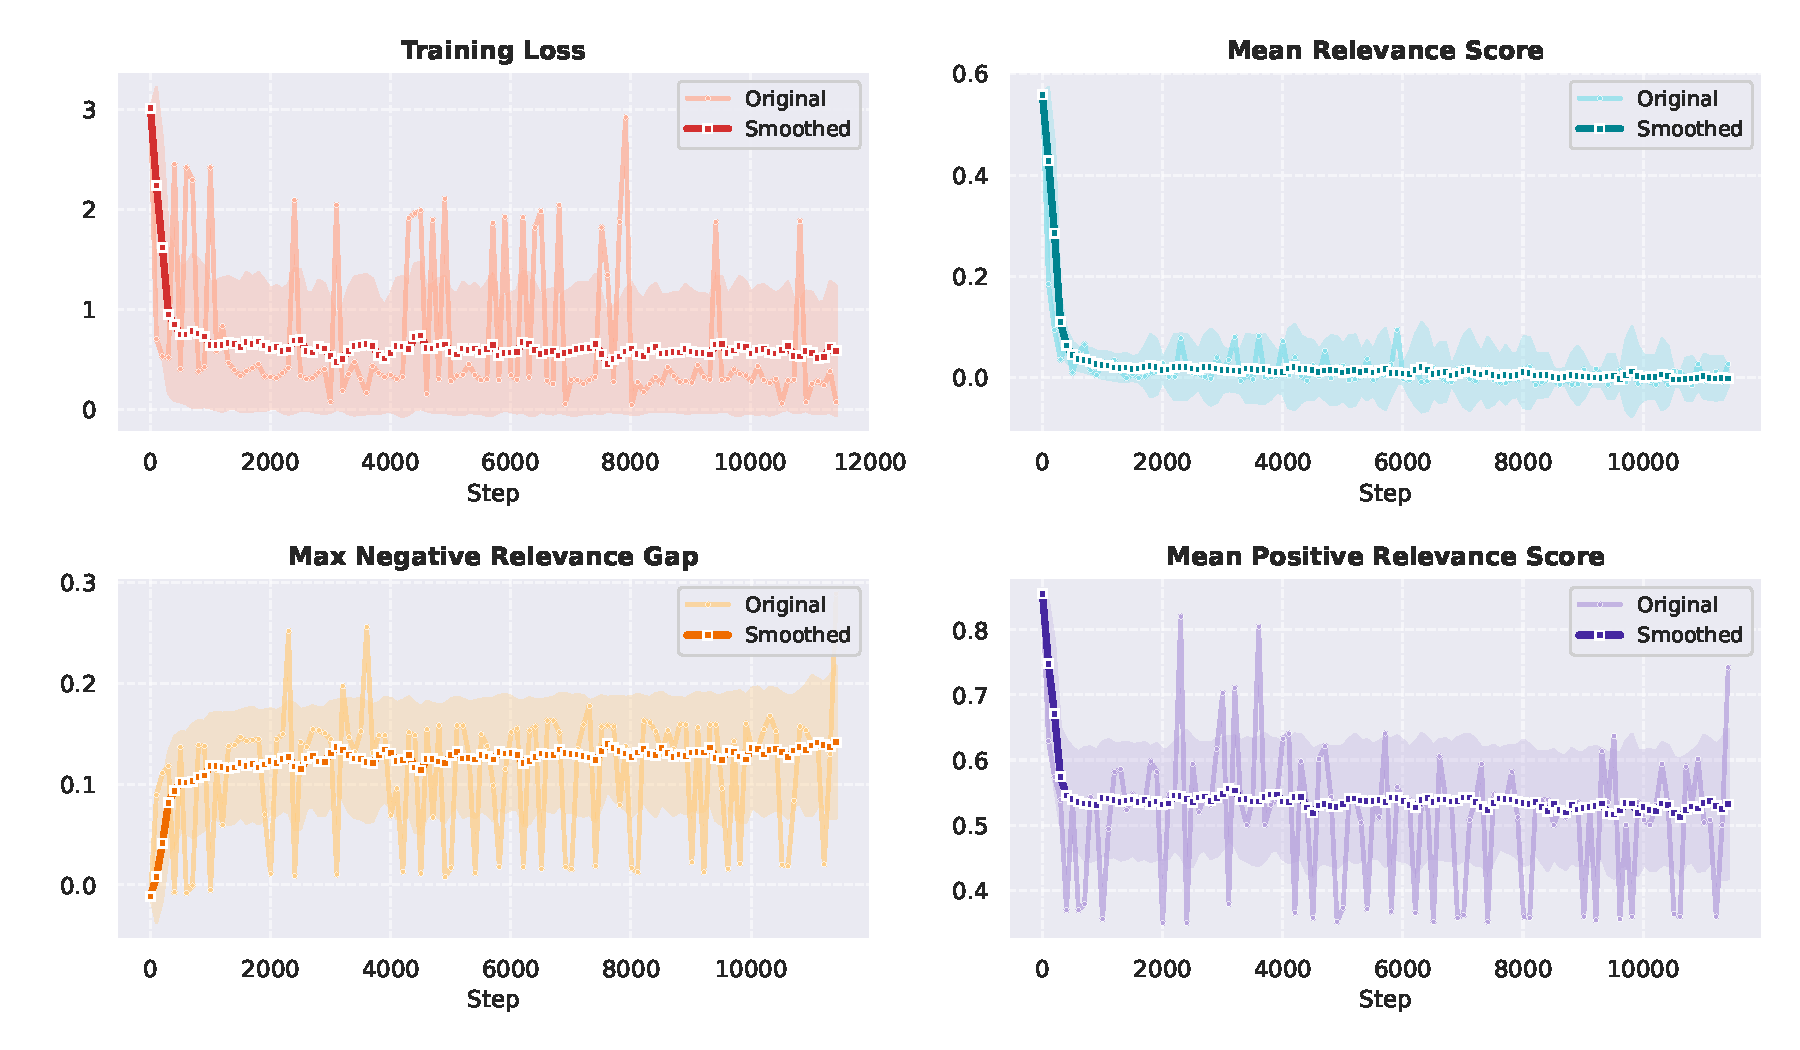
\includegraphics[width=\linewidth]{figures/gve/train_stat-qwen25vl_3b_all_0911.pdf}
    \caption{Training dynamics of \texttt{GVE-3B} across four metrics.}
    \label{gve:fig:train_3b}
\end{figure}

\begin{figure}[htbp]
    \centering
    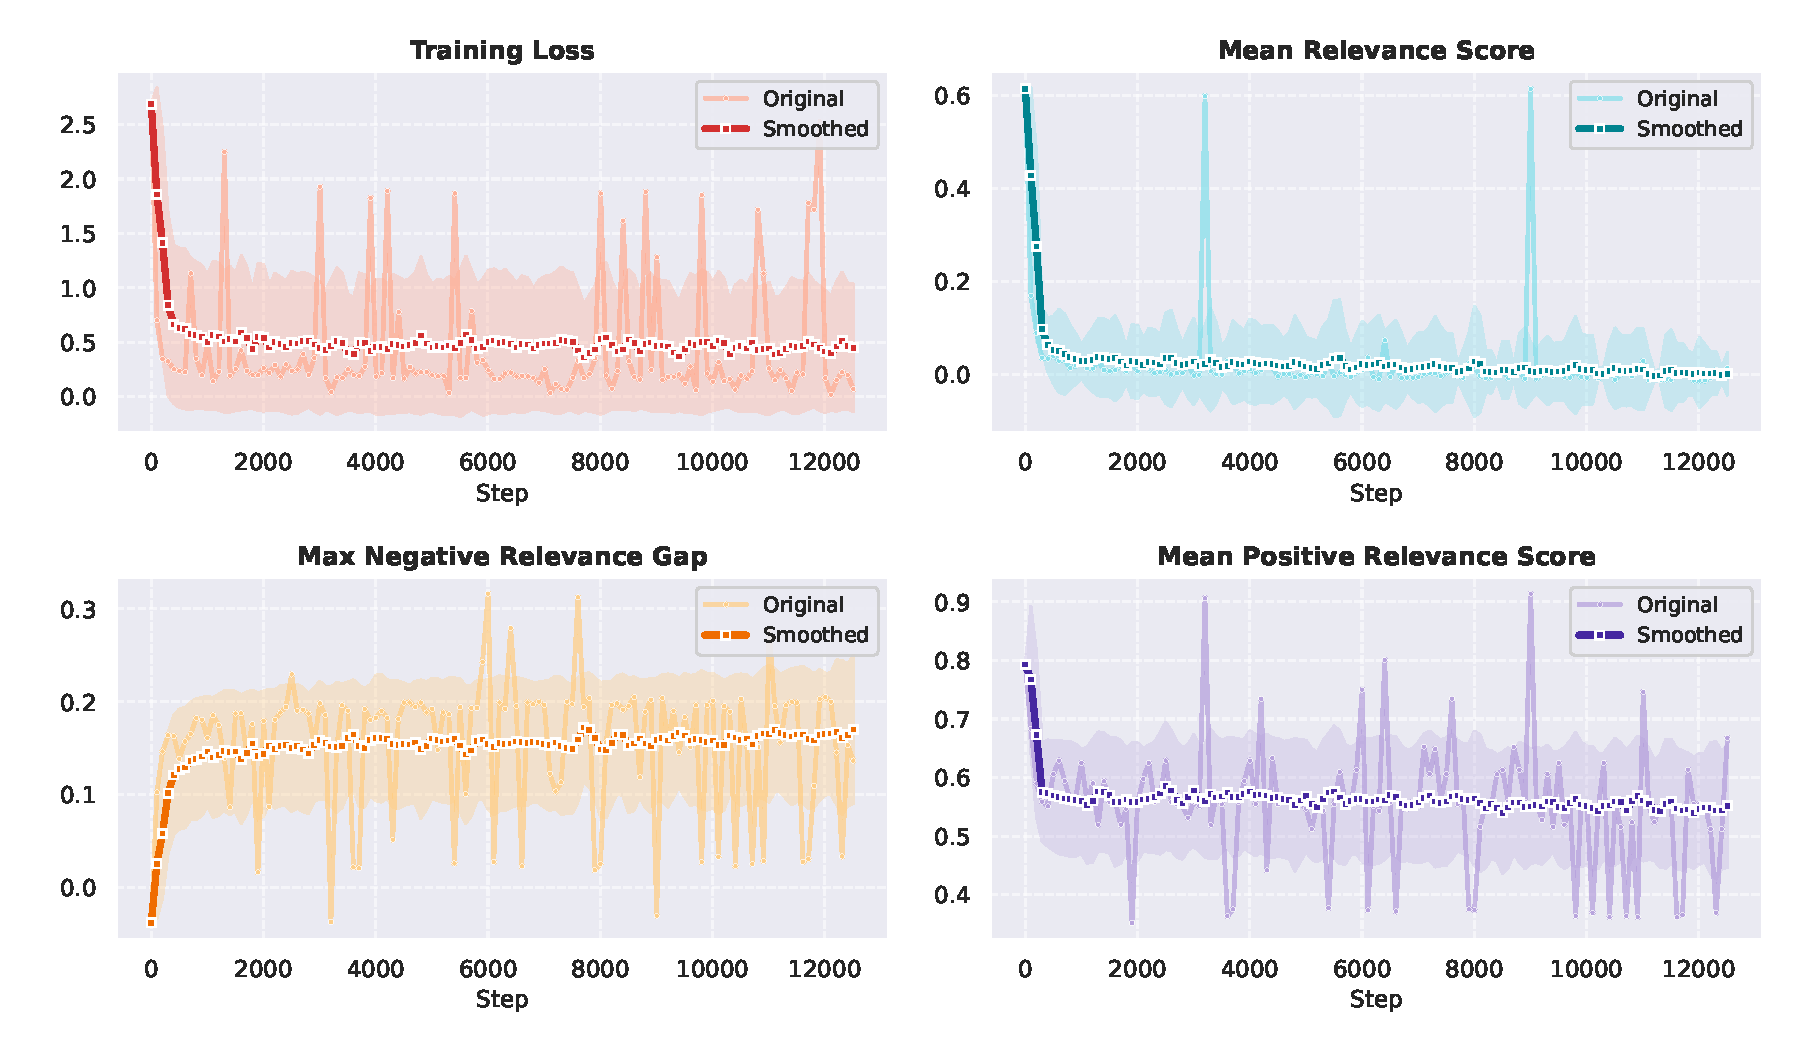
\includegraphics[width=\linewidth]{figures/gve/train_stat-qwen25vl_7b_all_0912.pdf}
    \caption{Training dynamics of \texttt{GVE-7B} across four metrics.}
    \label{gve:fig:train_7b}
\end{figure}














\subsection{Experiments of Training-time Scaling: More Results of Data Scaling}\label{gve:app:data_scaling}

Along with Section~\ref{gve:sec:data_scaling}, we depict more experiments for six abilities in data scaling for \texttt{GVE-3B} and \texttt{GVE-7B} in Figure~\ref{gve:fig:scaling_detail}. Shaded bands show $\pm1$ std; dashed curves are log-linear fits for visual guidance. X-axis is log-scaled to reflect scaling law dynamics.

\begin{figure}[htbp]
    \centering
    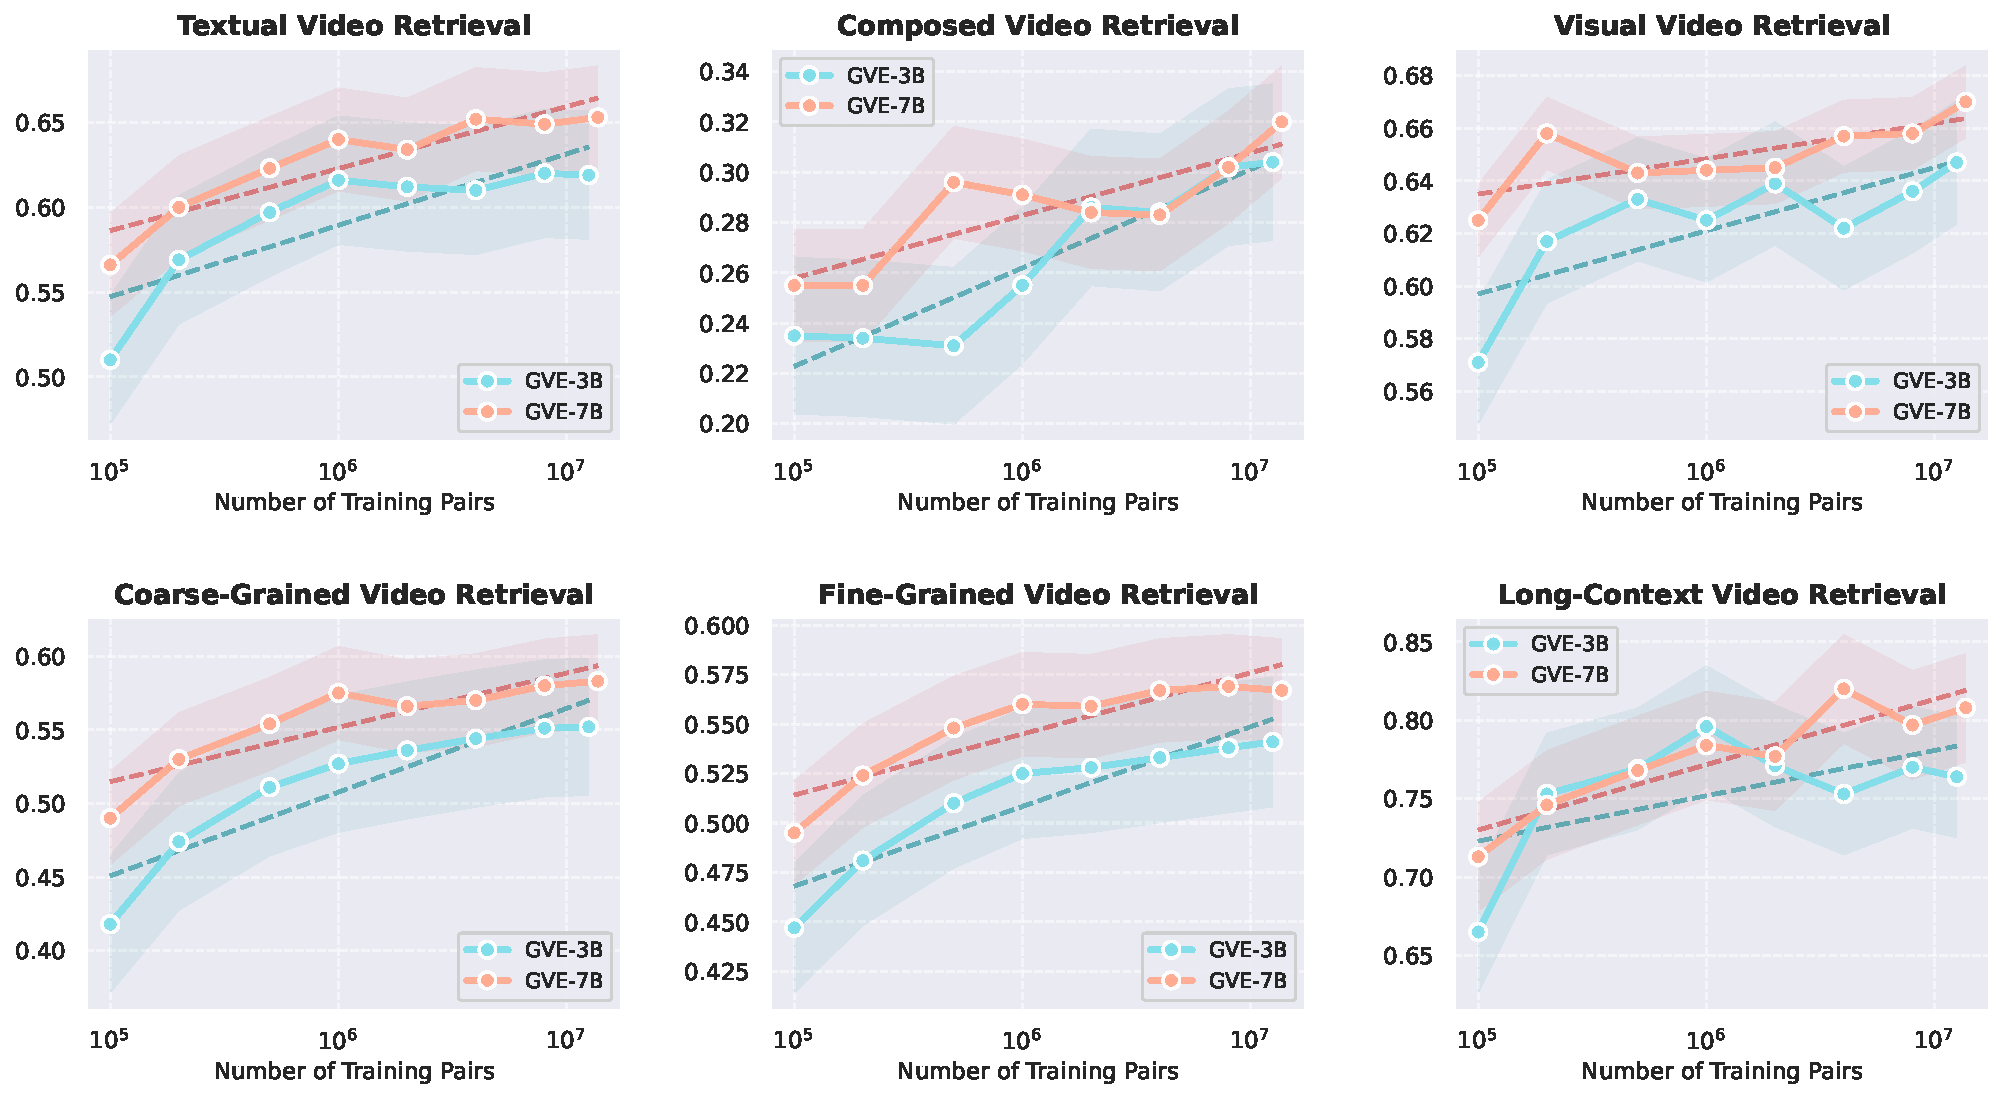
\includegraphics[width=\linewidth]{figures/gve/scaling_detail.pdf}
    \caption{Performance effect from data scaling for GVE-3B and GVE-7B in detail.}
    \label{gve:fig:scaling_detail}
\end{figure}

We fit a logarithmic scaling law $y = a \ln x + b$ to quantify gains per decade of data (10$\times$ increase). GVE-3B consistently shows higher relative gains: in compositional retrieval (CMP), it improves by $+0.039$ ($14.7\%$), nearly double GVE-7B’s $+0.025$ ($8.7\%$); in coarse-grained tasks (CG), it gains $+0.057$ ($11.1\%$), far exceeding GVE-7B’s $+0.037$ ($6.6\%$). Textual (TXT) and fine-grained (FG) retrieval follow similar trends, with GVE-3B improving by $+0.042$ ($7.1\%$) and $+0.040$ ($7.9\%$), respectively, versus GVE-7B’s $+0.037$ ($5.8\%$) and $+0.031$ ($5.6\%$). Visual retrieval (VIS) scales weakly for both ($+0.024$/$3.8\%$ for GVE-3B, $+0.013$/$2.1\%$ for GVE-7B). Notably, only in long-context retrieval (LC) does GVE-7B outperform GVE-3B in both absolute ($+0.042$ vs. $+0.029$) and relative gain ($5.4\%$ vs. $3.8\%$).

This reveals a task-dependent scaling trade-off: smaller models (GVE-3B) scale more efficiently in semantic and compositional tasks, while larger models (GVE-7B) uniquely excel in long-context modeling — suggesting that model size should be chosen not only for capacity, but for alignment with the data-scaling profile of the target task.



\subsection{Experiments of Test-time Scaling}\label{gve:app:scaling}

We investigate the impact of scaling two test-time parameters: the number of sampled frames and the maximum tokens per frame (i.e., effective resolution). We analyze each in isolation: when scaling the frame count from $8$ to $48$, the maximum token count is fixed at $200$; conversely, when scaling the token count from $200$ to $800$, the frame count is fixed at $8$.

\paragraph{Temporal Scaling: the Number of Sampled Frames.}

As shown in Figure~\ref{gve:fig:scaling_frame}, increasing the number of sampled frames generally improves performance. The most substantial gains appear in the Long-Context (LC) task (GVE-3B: +$19.6\%$, GVE-7B: +$12.8\%$), underscoring the value of denser temporal sampling for long-range reasoning. However, the Compositional (CMP) task shows a slight performance degradation, suggesting its sensitivity to potentially redundant visual cues from excessive frames. Furthermore, while GVE-7B consistently outperforms GVE-3B, the performance gap narrows as frames increase (from $0.029$ to $0.024$ on average scores across datasets), indicating that the larger model is more efficient at extracting information from sparser inputs.

\begin{figure}[htbp]
    \centering
    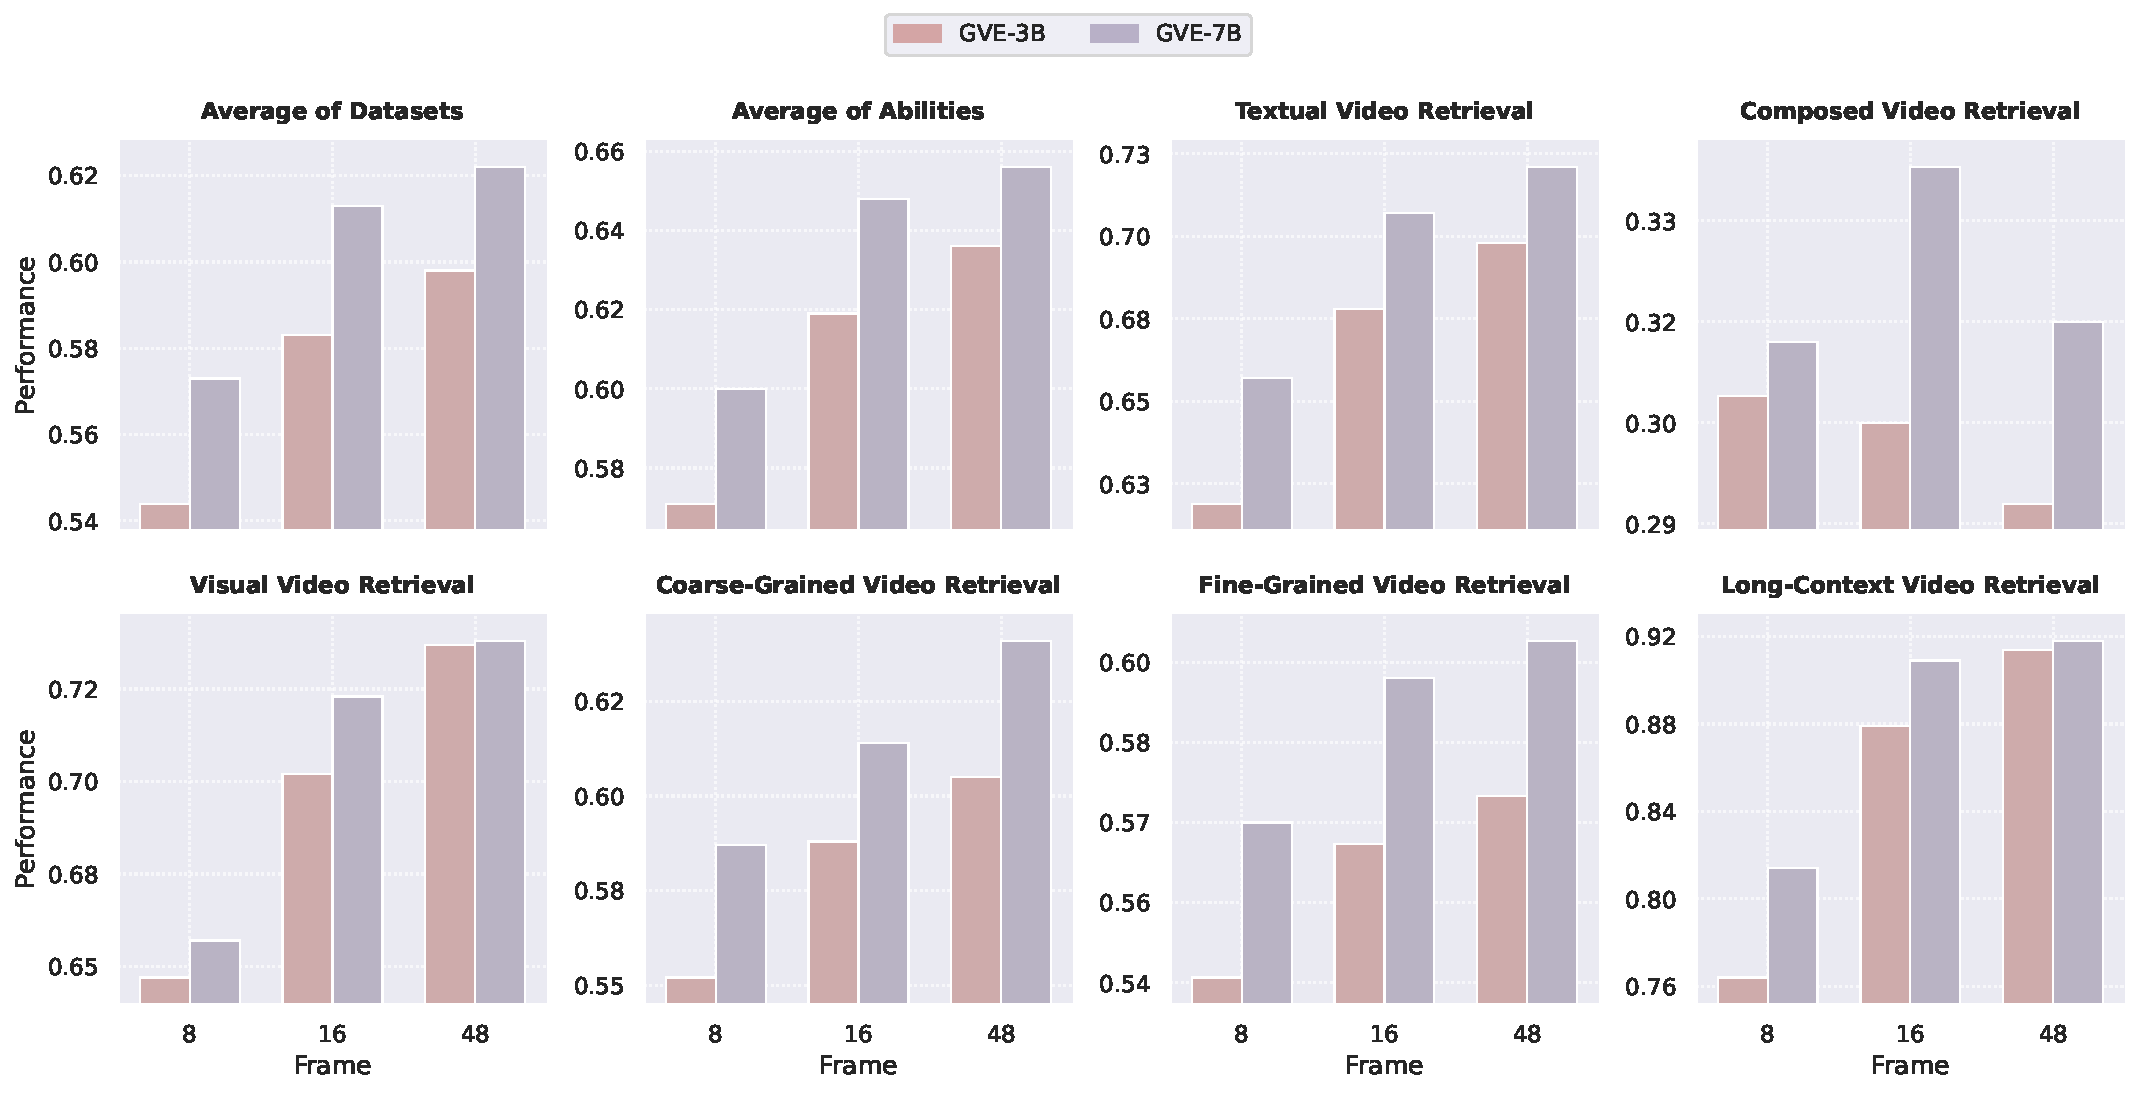
\includegraphics[width=\linewidth]{figures/gve/scaling_frame.pdf}
    \caption{Model performance as a function of the number of sampled frames at inference time (max tokens fixed at $200$).}
    \label{gve:fig:scaling_frame}
\end{figure}

\paragraph{Spatial Scaling: the Maximum Tokens Per Frame.}

In contrast, increasing the token budget yields non-monotonic returns (Figure~\ref{gve:fig:scaling_resolution}). Performance for most tasks peaks around $400$ tokens and then declines. This suggests that for semantic retrieval tasks, there is an optimal point of spatial detail. Scaling beyond this introduces a massive influx of fine-grained visual features that are largely redundant for the task. This over-saturation of information can dilute the effective semantic signal within the LLM's context window, making it more challenging for the model to distill the core visual concepts into the final embedding. The CMP task's performance again deteriorates with more tokens, reinforcing its sensitivity to input redundancy.

\begin{figure}[htbp]
    \centering
    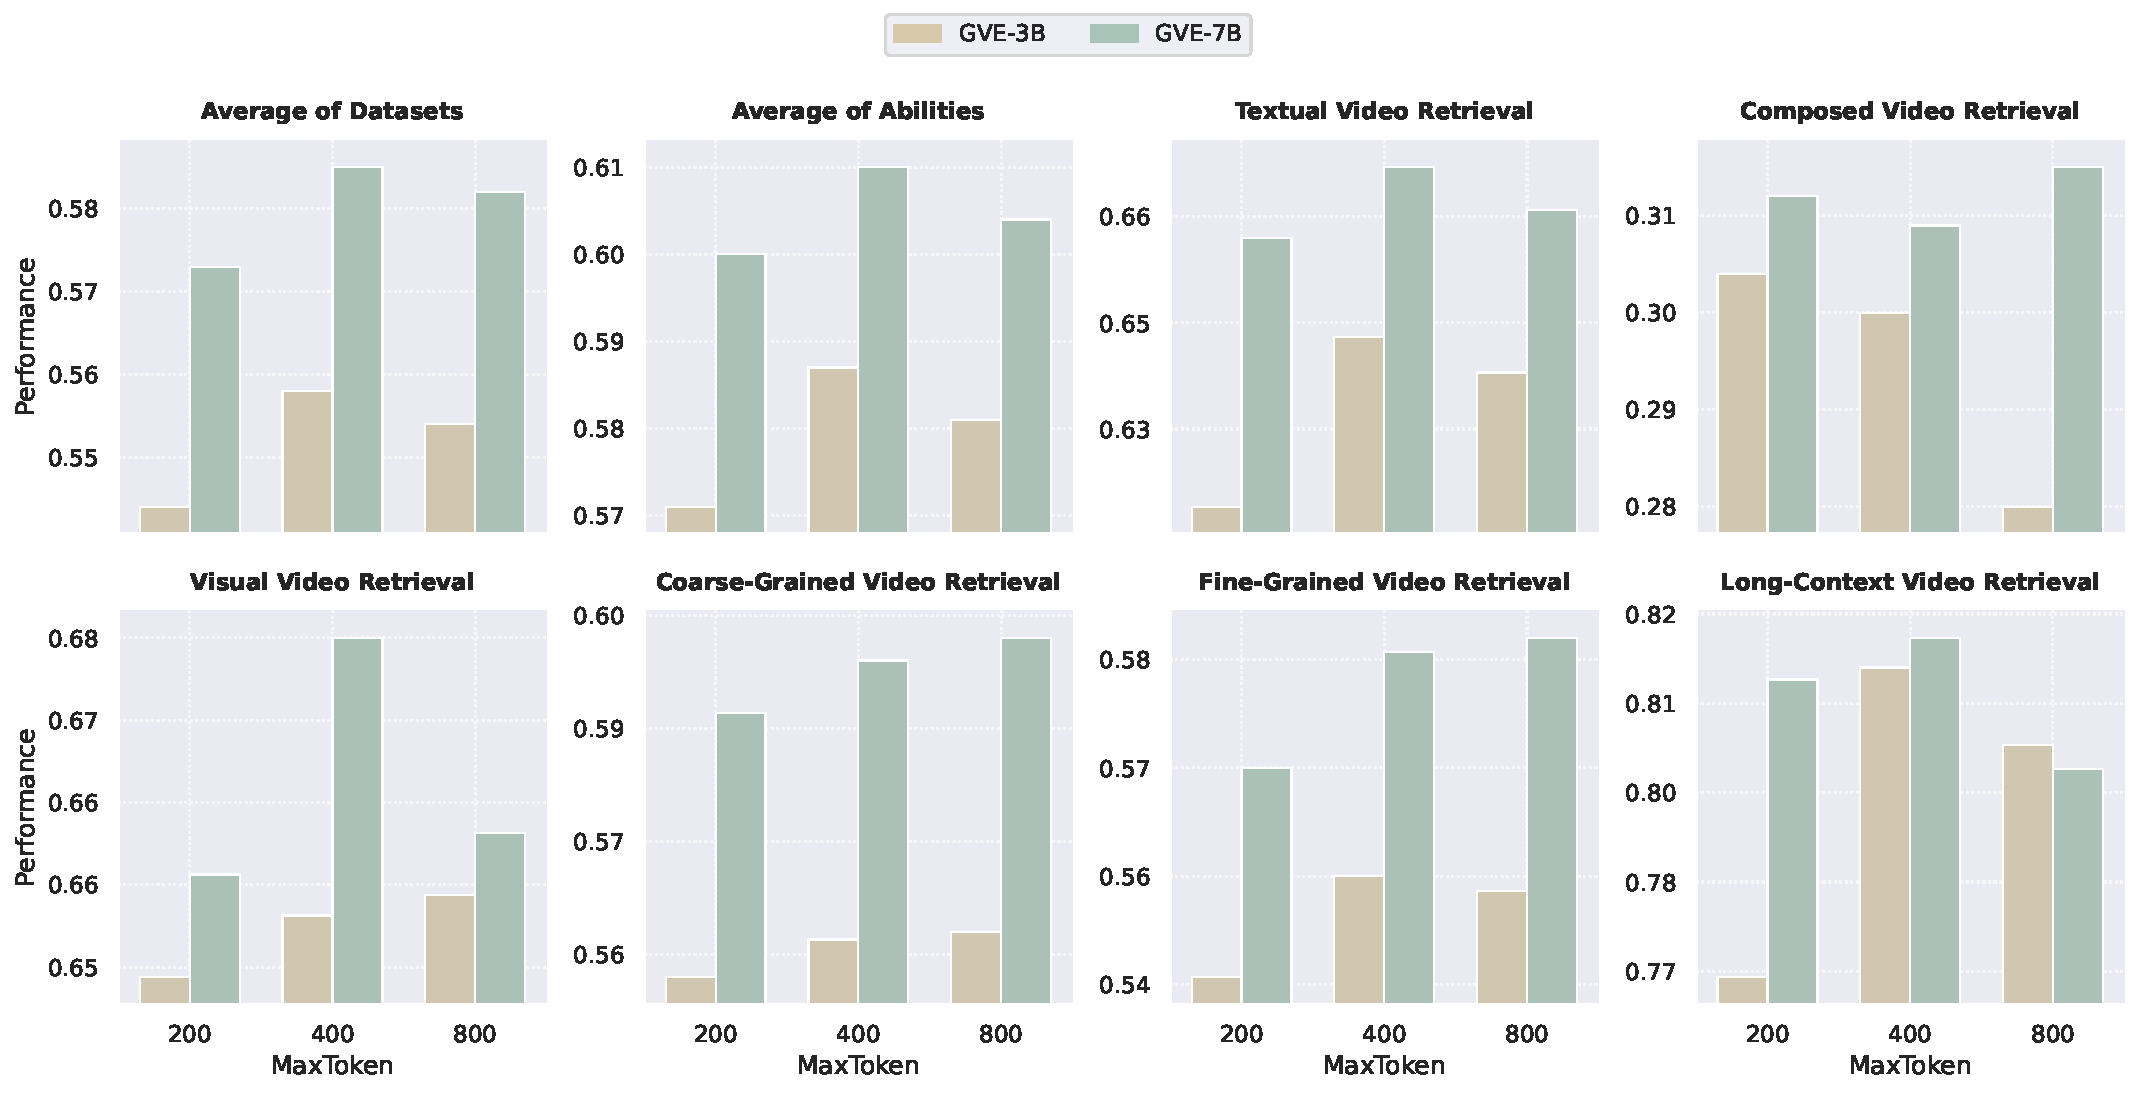
\includegraphics[width=\linewidth]{figures/gve/scaling_resolution.pdf}
    \caption{Model performance versus the maximum number of tokens per frame (frame count fixed at $8$), determining the resolution of frames in resizing.}
    \label{gve:fig:scaling_resolution}
\end{figure}

\paragraph{Key Findings and Implications.}

Our scaling analysis reveals four key findings:
\begin{itemize}
    \item \textbf{Temporal Scaling (More Frames):} Provides a reliable, though diminishing, performance boost, especially for long-range tasks.
    \item \textbf{Spatial Scaling (More Tokens):} Exhibits a clear optimal point (approx. $400$ tokens). Exceeding it degrades performance, indicating a trade-off between detail and distraction.
    \item \textbf{Model Scale Efficiency:} The larger model (GVE-7B) benefits less from input scaling, suggesting a greater intrinsic capacity to process sparse inputs effectively.
\end{itemize}

For test-time enhancement, temporal scaling is a robust strategy, whereas naive spatial scaling is not. This distinction underscores a critical insight: performance is not merely a function of total input data, but of its effective composition. It strongly motivates a shift from brute-force data scaling towards adaptive input mechanisms, such as dynamic token or frame selection, that can intelligently manage information density.



\subsection{Human-in-the-Loop Quality Validation of UVRD}\label{gve:app:v-synflow_validation}

To provide a ground-truth assessment of our synthesized data, we conducted a human expert evaluation on a random sample of $100$ instances generated from UVRD. As referenced in Section~\ref{gve:sec:data_synthesis}, the validation yielded a \textbf{$95\%$ factual accuracy rate}. The $5$ erroneous instances were categorized as follows, confirming they were minor and non-critical in nature:
$2$ instances with minor over/under-claims of visual details (e.g., recognize an object as a laptop/butterfly but it is not obvious);
$2$ instances with minor inaccuracies in camera motion description (e.g., movement hallucination);
$1$ instance with a subtle temporal sequencing error (e.g., reversed temporal description).
This high fidelity rate validates the effectiveness of our multi-stage quality assurance process in producing reliable training data at scale.


\subsection{Experimental Analysis of Modality Pyramid}\label{gve:app:pyramid_validation}

This subsection provides detailed experimental data to quantitatively validate the design choices and overall effectiveness of the \pyramid, as discussed in Section~\ref{gve:sec:modality_pyramid} and Section~\ref{gve:sec:ablation}.

\paragraph{Empirical Validation of Task Hierarchy}
The bottom-up design of our curriculum is predicated on an assumed hierarchy of task complexity. To empirically ground this assumption, we measured the initial alignment scores of different task types before training. We computed the average cosine similarity for $100$ positive pairs per task using the GME-7B~\cite{Zhang_2025_CVPR}. The results, presented in Table~\ref{gve:tab:task_alignment_appendix}, reveal a clear monotonic decrease in similarity as task complexity increases, from 0.68 for text-to-text (T2T) down to 0.43 for text-video-composed (TV2V) retrieval. This trend provides strong quantitative evidence for the assumed task hierarchy, justifying the curriculum's prioritization of foundational tasks.

\begin{table}[htbp]
\centering
\caption{Average cosine similarity of positive pairs across task types at initialization. The scores reveal a natural task difficulty hierarchy, providing an empirical basis for our curriculum design. T:~text, I:~image, V:~video.}
\label{gve:tab:task_alignment_appendix}
\footnotesize
\begin{tabular}{lcccccccc}
\toprule
Task Type & T2T & T2I & T2TI & I2TI & TI2TI & T2V & TI2V & TV2V \\
\midrule
Similarity & 0.68 & 0.65 & 0.59 & 0.53 & 0.52 & 0.46 & 0.45 & 0.43 \\
\bottomrule
\end{tabular}
\end{table}


\paragraph{Impact of Temperature Scheduling}
The curriculum's dynamic task scheduling is governed by a temperature parameter $\sigma(t)$ that increases linearly over time. To analyze its effectiveness, we compared this linear schedule against a fixed, manually tuned constant temperature ($\sigma = 0.5$) for GVE-3B. As shown in Table~\ref{gve:tab:temp_schedule_appendix}, the linear schedule achieves slightly superior final performance across datasets. This result suggests that an automated, adaptive scheduling mechanism can match or exceed a carefully tuned static hyperparameter, enhancing the robustness of the training process.

\begin{table}[htbp]
\centering
\caption{Performance comparison of temperature scheduling strategies at 3B scale.}
\label{gve:tab:temp_schedule_appendix}
\begin{tabular}{lc}
\toprule
Scheduling Strategy & Score \\
\midrule
Linear Schedule (Ours) & \textbf{0.571} \\
Constant Temperature ($\sigma=0.5$) & 0.569 \\
\bottomrule
\end{tabular}
\end{table}

\begin{table}[htbp]
\centering
\caption{Video classification accuracy comparison across different models and datasets. For each column: highest score is \textbf{bolded}, second-highest is \underline{underlined}.}
\label{gve:tab:video_classification}
\begin{tabular}{@{}l|>{\columncolor{gray!15}}c|*{5}{c}@{}}
\toprule
\textbf{Model} & \textbf{AVG} & \textbf{K700} & \textbf{UCF101} & \textbf{HMDB51} & \textbf{SSV2} & \textbf{Breakfast} \\
\midrule
CLIP4Clip       & 0.378 & 0.395 & 0.596 & 0.413 & 0.308 & 0.176 \\
InternVideo2-6B & \textbf{0.526} & \textbf{0.554} & 0.572 & 0.480 & \textbf{0.569} & \textbf{0.453} \\
VLM2Vec-V2      & 0.393 & 0.380 & 0.600 & 0.409 & 0.428 & 0.148 \\
GME-7B          & 0.374 & 0.397 & 0.547 & 0.479 & 0.306 & 0.143 \\
UniME-7B        & 0.306 & 0.388 & 0.377 & 0.407 & 0.190 & 0.166 \\
Unite-7B        & \underline{0.519} & 0.537 & \underline{0.752} & \textbf{0.534} & 0.513 & 0.261 \\
\midrule
GVE-3B          & 0.476 & 0.489 & 0.661 & 0.483 & 0.471 & 0.277 \\
GVE-7B          & \textbf{0.526} & \underline{0.540} & \textbf{0.757} & \underline{0.525} & \underline{0.521} & \underline{0.289} \\
\bottomrule
\end{tabular}
\end{table}

The effectiveness of this linear schedule lies in its data-driven nature. The prober model implicitly determines task difficulty based on alignment scores, leading to an adaptive schedule without requiring manual prior assumptions about which tasks are inherently ``harder.'' We believe this data-driven approach is more robust for a universal framework than hand-crafted, task-specific schedules.





\subsection{Experiments of Video Classification}\label{gve:app:video_classification}

We test the video embeddings for video classification by following the MMEB-V2~\cite{meng2025vlm2vec}.
Note that we do not train on these datasets for zero-shot evaluations, while other baselines may include them in optimization.
Specifically, we evaluate video embedding models on five diverse classification benchmarks, including \textbf{Kinetics-700~(K700)}~\cite{carreira2019short}, \textbf{UCF101}~\cite{soomro2012ucf101}, \textbf{HMDB51}~\cite{kuehne2011hmdb}, \textbf{SomethingSomething-V2~(SSV2)}~\cite{goyal2017something}, and \textbf{Breakfast}~\cite{kuehne2014language}, covering fine-grained interactions, open-domain actions, and procedural activities. Each task is cast as video-to-text retrieval over the full label set, using standardized validation/test splits.
The results are provided in Table~\ref{gve:tab:video_classification}.
Our results show that \texttt{GVE-7B} and \texttt{InternVideo2-6B} achieve the highest mean accuracy ($0.526$), demonstrating the efficacy of unified multimodal representations. However, performance remains suboptimal on temporally complex datasets such as Breakfast (best: $0.453$) and fine-grained SSV2 (best: $0.569$), revealing a critical bottleneck in modeling dynamic physical interactions.
